% calculus:x21 GDC:YES
\begin{question}
  \hspace*{\fill} [Note maximale: 6]\par
  \noindent Soit $f(x) = e^x Sin 2x + 10$, avec $0 \le x \le  4$.  Une partie de la représentation graphique de $f$ est donnée ci-dessous.\par
  \medskip
  \begin{center}
    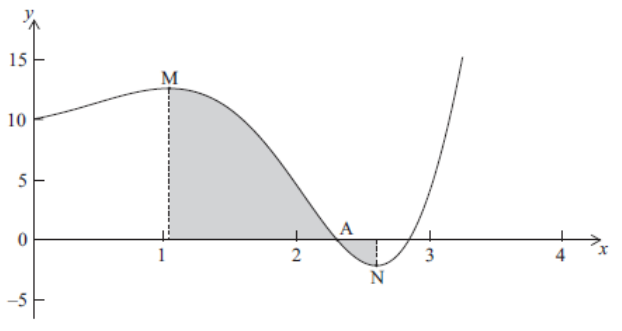
\includegraphics[scale=0.25]{etox_sin2x}\par
  \end{center}
  \noindent Sont représentés une abscisse a l'origine au point $A$, un maximum relatif au point $M$ avec $x = p$ et un minimum relatif au point $N$ avec $x = q$.\par
  \medskip
  (a) Donnez les abscisses de $A$.\hspace*{\fill} [1]\par
  \medskip
  (b) Trouvez la valeur de\par
  \hspace{1em} (i ) $p$\par 
  \hspace{1em} (ii) $q$\hspace*{\fill} [2]\par
  \medskip
  (c) Trouvez $\int_p^qf(x)dx$. Expliquez pourquoi ceci n'est pas l'aire de la région grisée.\hspace*{\fill} [3]\par
\end{question}
